\chapter{Regions of interest}

The regions of interest (ROI) were chosen as pixel locations in the image on specific places of the hand. ROI were selected on behalf of getting a full representation of the hand, to investigate the regions which show the most significant difference when computing the statistical test. 
Regions in the fingertips and nail folds are areas where it is easy to access the microcirculatory hemodynamics of the human body according to \cite{Iabichella2006}. This region should therefore be expected to give some information on the changes in capillaries which can be an effect of vasomotion. 

The original image \ref{fig:hand} is showing the hand but not with very good contrast. To easier choose ROI, the original image was converted to a gray scale image to improve the contrast in the image, this can be seen in \ref{fig:mat2grayHand}. 

\begin{figure}[H]
	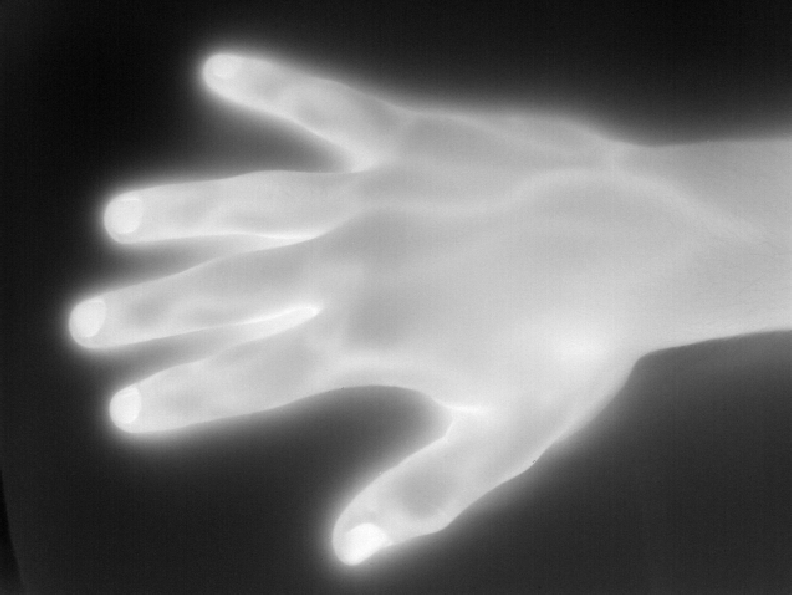
\includegraphics[width=0.5\textwidth]{figures/mat2grayHand}  %<--but is not needed.
	\caption{First thermal image of the thermal image series for subject 1, grayscale image}
	\label{fig:mat2grayHand}  %<--give the figure a label, so you can reference!
\end{figure}

With the improved contrast, 28 ROI from the hand were chosen on the first image of the thermal image series, by finding the coordinates of the pixels on the image. The regions are illustrated on \ref{fig:roiHand}. The localization of the regions is originating from the fingertips and elongating down the hand to the beginning of the wrist. Each region gives an pixel intensity value from one pixel of the image. Further more the mean of the chosen pixel value and the neighbor pixels, a total  of nine pixels, is calculated for each region to get a more general value for the specific region.

\begin{figure}[H]
	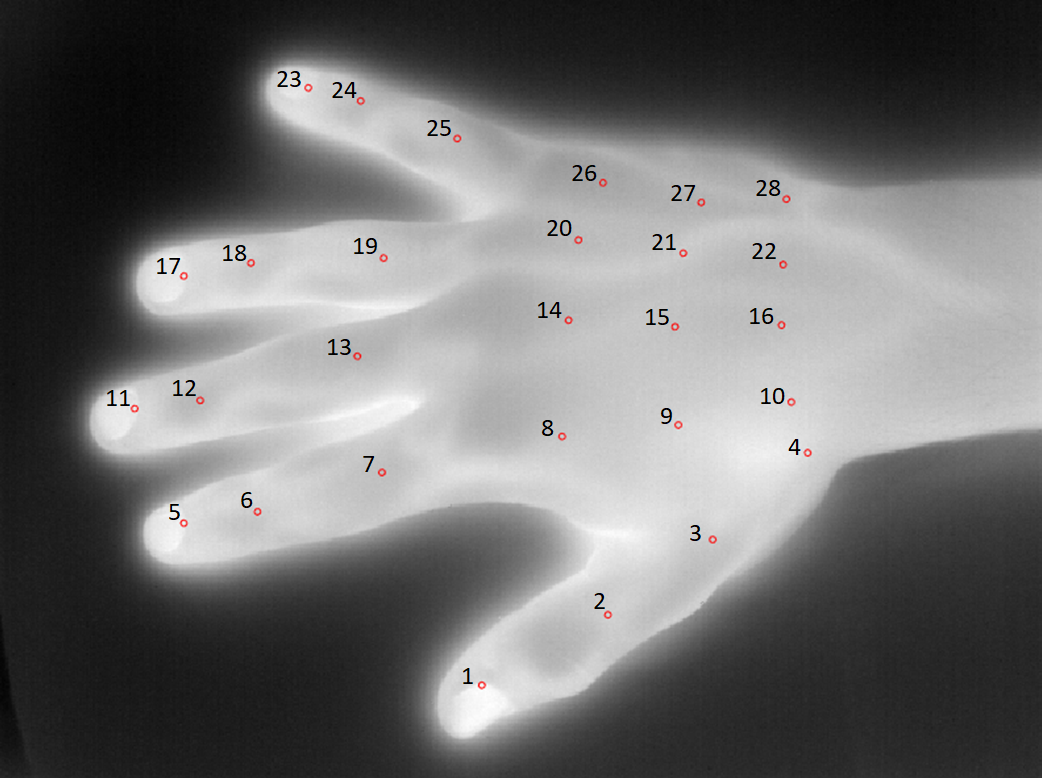
\includegraphics[width=0.5\textwidth]{figures/roiHand}  %<--but is not needed.
	\caption{First thermal image of the thermal image series for subject 1, with ROI of interest plottet on 28 areas of the hand represented as red circles}
	\label{fig:roiHand}  %<--give the figure a label, so you can reference!
\end{figure}

The regions are constant for the whole image series for each measurement, assuming that the subject was sitting still during the whole measurement. The regions also account for both the uncuffed and cuffed conditions for each subject, assuming that the position of the hand was at the same position in both conditions. 
Iterating over the image series saving ROI into a cell array with data points for each ROI, a vector for the each of the 28 regions was made to give the pixel intensity variations over the whole measurement. 
An example of the pixel intensities for one subject is shown on image \ref{fig:Intensities}

\begin{figure}[H]
	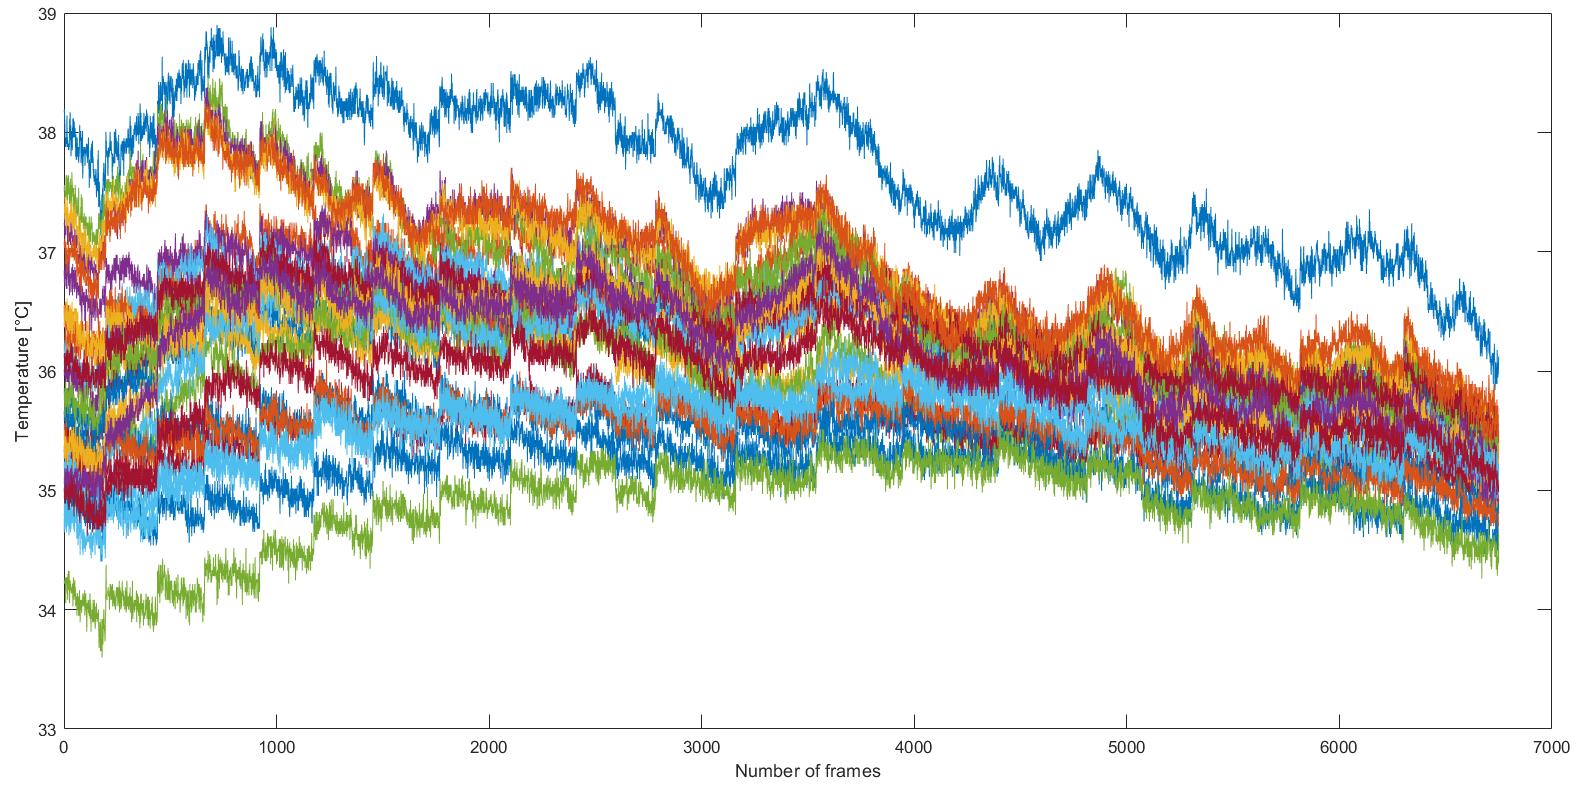
\includegraphics[width=1\textwidth]{figures/Intensities}  %<--but is not needed.
	\caption{Pixel intensity for all 28 ROI, plottet from subject 1, for the entire thermal image series of a measurement}
	\label{fig:Intensities}  %<--give the figure a label, so you can reference!
\end{figure}

It is noticed that there are some jumps at specific times in the pixel intensity for all ROI, this is due to the drift auto correction from the camera shutter \fixme{a citation of reference to another place should be here for documentation}. This problem is dealt with in the next section. %something like that...? dunno if it is to much to take the intensity plot with here? but i was thinking it to be to make a smooth transition to the drift correction... 